\chapter{Ejemplo de Uso del Proyecto}

Esta tesis se centra tanto en el riesgo como en el desarrollo de un Chatbot, este chatbot funciona 
en base a la una arquitectura de RAG (Retriever-Augmented Generation) por lo que esta consiste en 
la recuperación de contexto el cual es enviado junto con el prompt al LLM. El proceso comienza con 
la obtención de un prompt específico del usuario, tal como ``Dame un resumen del documento Dominga'' 
dentro de la barra de búsqueda del frontend. Este prompt actúa como entrada inicial para el sistema 
de recuperación de información.

%\begin{figure}[ht!]
%    \centering
%    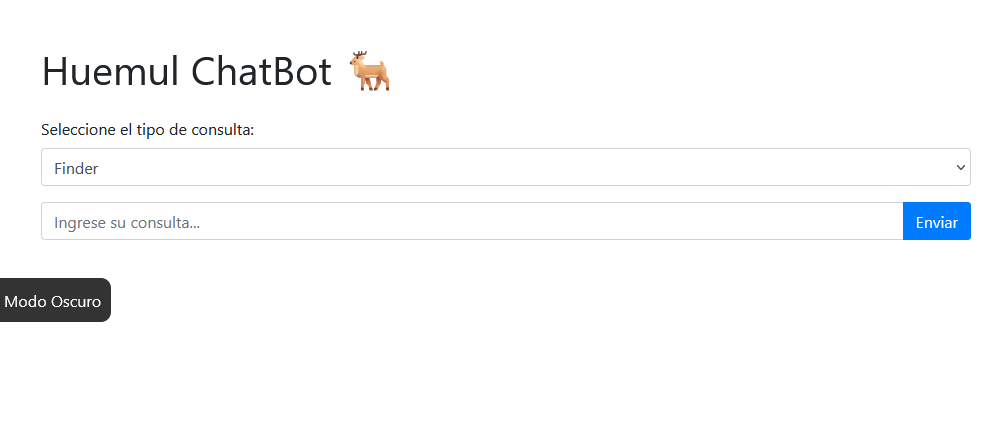
\includegraphics[width=.8\textwidth]{figures/website.png}
%    \caption[]{\\
%    {\scriptsize (Fuente: Elavoración propia)}}
%    \label{fig:chatbot1}
%\end{figure}

El prompt se procesa mediante una función de Embedding, empleando para ello OpenAI, siendo esta  
la función 'text-embedding-ada-002'. Esta función puede manejar hasta un máximo de 8191 tokens y 
produce un vector de 1536 dimensiones en forma de lista \cite{openai1}. Para determinar la similitud entre el 
vector del prompt y los vectores correspondientes a los documentos almacenados, se utiliza la función 
de similitud coseno presente en la \autoref{eq:similitudcoseno}.Esta mide el coseno del ángulo entre dos vectores,
Siendo estos $A$ y $B$ respectivamente, y este proporciona un valor que refleja su proximidad semántica entre el vector
del prompt y los vectores de todos los documentos almacenados en la base de datos ChromaDB.

\begin{equation}
    \text{similitud\_coseno}(\mathbf{A}, \mathbf{B}) = \frac{\mathbf{A} \cdot \mathbf{B}}{\|\mathbf{A}\| \|\mathbf{B}\|}
    \label{eq:similitudcoseno}
\end{equation}


El proceso de embedding como se menciono antes lo que realiza en otras palabras es la conversión de un texto a un vector, esto debido a que los modelos de LLM al ser basados 
en redes neuronales necesitan un presentación grafica de estos texto a un formato el cual pueda ser legible por el modelo, por lo que se convierten en números como muestra la 
\autoref{fig:caso1} a continuación.

\begin{figure}[ht!]
    \centering
    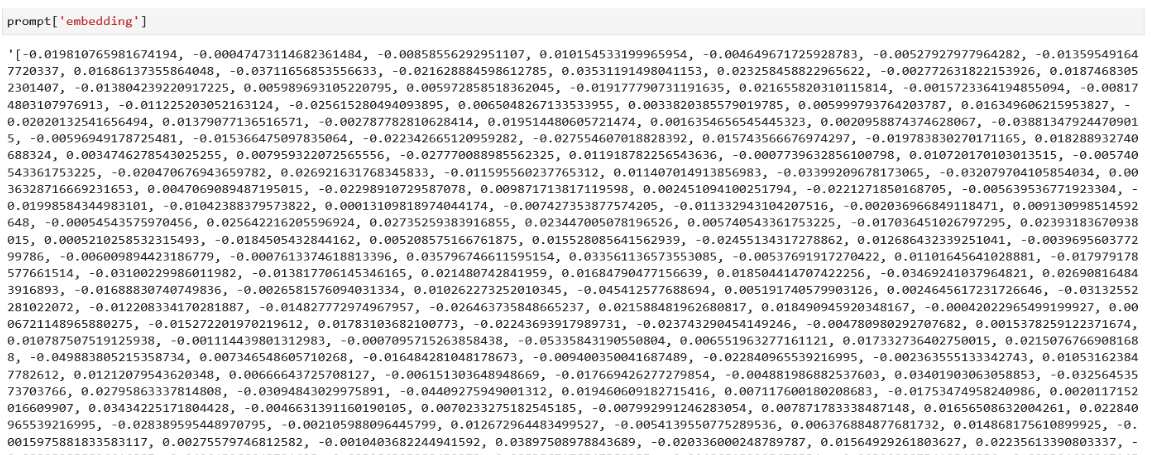
\includegraphics[width=0.7\textwidth]{figures/embedding1.png}
    \caption[Representación vectorial de un prompt luego de pasar por la funcion de embedding]{Representación de un prompt luego de pasar por la funcion de embedding 'text-embedding-ada-002'\\
    {\scriptsize (Fuente: Elavoración propia)}}
    \label{fig:caso1}
\end{figure}

\newpage

Una vez calculada la similitud coseno entre el vector asociado al prompt y los vectores que presentan los documentos que se encontraban en la 
base de datos, se procede a elaborar un ranking de los documentos más relevantes, según la similaridad obtenida del cálculo de similitud de cosenos. 
Esto se realiza seleccionando los 'n' documentos con los valores de similitud más altos, siendo en el ejemplo proporcionado un total de 3 
presente en la \autoref{fig:caso2}.

\begin{figure}[ht!]
    \centering
    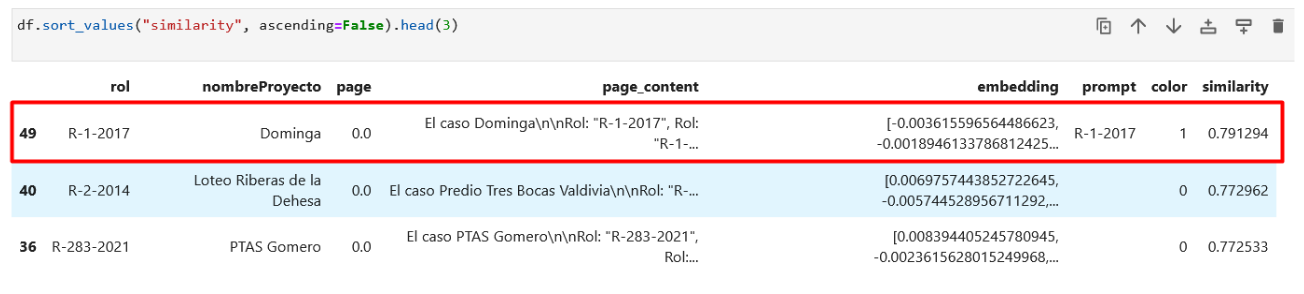
\includegraphics[width=1\textwidth]{figures/embedding2.png}
    \caption[Screenshot de un jupyter notebook representando el proceso interno de selección]{Screenshot de un jupyter notebook representando el proceso interno de selección\\
    {\scriptsize (Fuente: Elavoración propia)}}
    \label{fig:caso2}
\end{figure}

Todo este proceso funciona internamente usando Langchain que consulta estos ‘n’ documentos, siendo en este caso 3, a la base de datos 
ChormaDB y son enviados como contexto dentro del prompt a OpenAI mediante el uso de su API, junto a la key de autorización, 
para obtener el resultado del modelo.

Finalmente, se obtiene el resultado por parte del modelo y es procesado por el frontend de la forma que se observa en la \autoref{fig:caso3}, 
lo que da fin al proceso que realiza el Chatbot de principio a fin.


\begin{figure}[ht!]
    \centering
    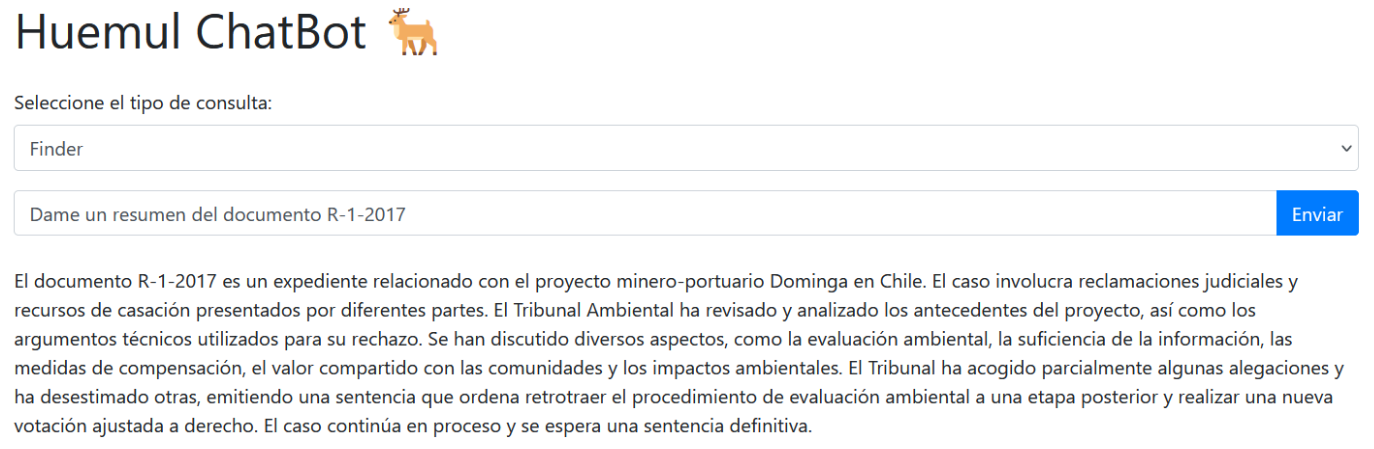
\includegraphics[width=0.95\textwidth]{figures/website2.png}
    \caption[Screenshot del funcionamiento del Chatbot]{Screenshot del funcionamiento del Chatbot\\
    {\scriptsize (Fuente: Elavoración propia)}}
    \label{fig:caso3}
\end{figure}